\documentclass[12pt]{report}

%%%%%%%%%%%%%%%%%%%%%%%%%%%%%%%%%%%%%%%%%%%%%%%%%%%%%%%%%%%%%%%%%%%%%%%%

\usepackage{lmodern}        % use modern latin fonts
\usepackage[T1]{fontenc}    % use 8 bit output font encoding with more glyphs
\usepackage[utf8]{inputenc} % so you can type ă

\usepackage{xcolor}         % more color choices
\usepackage[english=british]{csquotes} % for correct use of `` '' ... TODO!!
\usepackage{url}            % typeset URL's sensibly
\usepackage{enumitem} % configure labels of items in enumerations i.e. i), ii)
\usepackage[nottoc]{tocbibind} % include bibliography in ToC (third-rep.cls not working)
\usepackage{appendix} % customise the appearance of appendix via an 'appendix' environment
\usepackage{float}
\usepackage{tabu}

\usepackage[a4paper,textwidth=159mm, hmargin ratio=1:1, vmargin ratio=1:1, verbose]{geometry}
\makeatletter
\AtEndPreamble{%
  \normalfont
  \ifcase \@ptsize
    \geometry{textheight=240mm}%
    \or
    \geometry{textheight=243mm}%
    \or
    \geometry{textheight=241mm}%
  \fi
}

\usepackage{natbib}
\setcitestyle{authoryear,round}

%% =============================================================================
% Remove "Chapter x" line before a new chapter
% This should be in .cls file, ideally
\makeatletter
\renewcommand{\@makechapterhead}[1]{%
  % \vspace*{15 pt}% Space before the chapter name
  {\setlength{\parindent}{0pt} \raggedright \normalfont
    \bfseries\Huge
    #1% The chapter's name
    \par\nobreak\vspace{35 pt}}} % Space after chapter name
\makeatother
%% =============================================================================

\usepackage{amsmath, amssymb}
\DeclareMathOperator*{\argmin}{argmin}
\providecommand{\norm}[1]{\lVert#1\rVert}

\usepackage{graphicx}
\graphicspath{{./images/}}

\usepackage{caption,subcaption}
% \subref -> '(a)' rather than just 'a'
\captionsetup[subfigure]{subrefformat=simple,labelformat=simple}
\renewcommand\thesubfigure{(\alph{subfigure})}
\makeatletter
\renewcommand\p@subfigure{\thefigure~}
\makeatother

\usepackage[backref]{hyperref}
\hypersetup{
  pdftitle      = {TODO},
  pdfauthor     = {Ciprian Tomoiaga},
  pdfsubject    = {TODO},
  pdfkeywords   = {TODO},
  pdfpagemode   = UseOutlines,
  pdfstartview  = Fit,
  pdfpagelayout = OneColumn,       % document in 1 column continuous scrolling
  unicode=true,                    % use Unicode in bookmarks
  bookmarksnumbered  = true,       % shows numbers in bookmarks like ToC
  bookmarksopen      = true,
  bookmarksopenlevel = 1,
  colorlinks   = true,             % Colours links instead of ugly boxes
  urlcolor     = {blue!80!black},  % Colour for external hyperlinks
  linkcolor    = {red!50!black},   % Colour of internal links
  citecolor    = {blue!50!black},  % Colour of citations
  breaklinks   = true,             % Break long links into lines
  linktocpage  = false             % ToC, LoF, LoT place hyperlink on page number, rather than entry text
}

%% ----------------------------------------------------------------------------
\newcommand*{\nolink}[1]{%
  \begin{NoHyper}#1\end{NoHyper}%
}

%% ----------------------------------------------------------------------------
\newcommand{\algorithmautorefname}{algorithm}
% TODO: workaround incompatibility hyperref + appendix package
% \newcommand{\appref}[1]{\hyperref[#1]{Appendix~\ref{#1}}}


%% ----------------------------------------------------------------------------
% provide \Autoref :
\usepackage{catoptions}
\makeatletter
\def\figureautorefname{figure}
\def\tableautorefname{table}
\def\Autoref#1{%
  \begingroup
  \edef\reserved@a{\cpttrimspaces{#1}}%
  \ifcsndefTF{r@#1}{%
    \xaftercsname{\expandafter\testreftype\@fourthoffive}
      {r@\reserved@a}.\\{#1}%
  }{%
    \ref{#1}%
  }%
  \endgroup
}
\def\testreftype#1.#2\\#3{%
  \ifcsndefTF{#1autorefname}{%
    \def\reserved@a##1##2\@nil{%
      \uppercase{\def\ref@name{##1}}%
      \csn@edef{#1autorefname}{\ref@name##2}%
      \autoref{#3}%
    }%
    \reserved@a#1\@nil
  }{%
    \autoref{#3}%
  }%
}
\makeatother



% \usepackage{algpseudocode}
% \usepackage{algorithmicx}
% \algrenewcommand{\algorithmiccomment}[1]{\hskip3em// #1}
%\renewcommand{\algorithmicforall}{\textbf{for each}} % 'for all' -> 'for each'
% define commands to indent without \State
% \algdef{SE}[SUBALG]{Indent}{EndIndent}{}{\algorithmicend\ }%
% \algtext*{Indent}
% \algtext*{EndIndent}


% typeset the name of a package: \pkg{tum_ardrone}
\newcommand{\pkg}[1]{\textsf{\detokenize{#1}}}


\title{Handwriting recognition in business documents}
\author{Ciprian Ioan Tomoiagă}


%\usepackage{fancyhdr}
%\pagestyle{fancy}
%\lhead{}  % left head
%\chead{Draft: \today} % centre head
%\lfoot{}
%\cfoot{\thepage}
%\rfoot{}

\renewcommand{\bibname}{References} % Bibliografy -> References

\begin{document}

% %!TEX root = ../main.tex
% make \today be Month, year
\renewcommand{\today}{\ifcase \month \or January\or February\or March\or %
April\or May \or June\or July\or August\or September\or October\or November\or %
December\fi, \number \year}

\makeatletter
\begin{titlepage}
  \begin{center}
    \vspace*{2cm}

    \rule{.9\linewidth}{.6pt}
    {\huge \textbf{\@title}\par}
    \rule{.9\linewidth}{.6pt}

    {\large Master's project \par}
  \end{center}

  \vspace{7cm}
  \begin{minipage}[t]{.5\textwidth}
    \large
    \textit{Author:}

    \textbf{\@author}
  \end{minipage}
  \begin{minipage}[t]{.4\textwidth}
    \large
    \raggedleft
    \textit{Supervisors}:

    \textbf{Dr. Mathieu Salzmann}
    \textbf{Patrick Jayet}
  \end{minipage}

  \begin{center}
  \vspace{\fill}
  \textit{\today}
  \vspace{\fill}

  
\includegraphics[width=0.3\textwidth]{epfl_logo}
  \end{center}
\end{titlepage}
\makeatother

% \thispagestyle{empty}
\vspace*{1cm}

\centerline{\Large\textbf{Abstract}}

\large
	This project is a first step in information extraction from complex, heterogeneous and handwritten business forms, with the aim of speeding up their processing. It tackles the main problems of handwriting detection and recognition in the challenging context of no labelled data.

	Our work adapts well known deep learning architectures in order to solve each of them separately, namely the successful Faster R-CNN for detection and the Convolutional Recurrent Neural Networks for transcription. We carry out several experiments on each task which prove that we can greatly benefit from transfer learning to avoid the high cost of data labelling. In addition, we show new data generation techniques which further help in this regard and which allow us to inspect the important factors that influence the model's performance.

	Finally, we assemble the two parts together into a proof of concept system that is able to detect handwritten text in highly challenging documents and to transcribe some of it correctly.

\normalsize

% \newpage
\vspace*{3.5cm}

\centerline{\Large\textbf{Acknoledgements}}\bigskip

\large
I would like to express my deep gratitude to Dr Mathieu Salzmann for his guidance, valuable advice and fruitful discussions. His willingness to give his time so generously has been very much appreciated.

I am also particularly grateful for the assistance given by Patrick Jayet and for his lessons in solving problems pragmatically. My special thanks are extended to the staff of AXA Engineering lab for sharing their expertise with me and for making the office a great place to learn.

Finally, I wish to thank Ana Ciolan and my family for their continuous support and encouragement throughout my studies.

\normalsize


\tableofcontents
\listoffigures
% \listoftables


%% These include the actual text
%!TEX root = main.tex
% Chapter 1

\chapter{Introduction} % Main chapter title

\label{ch:intro}

%----------------------------------------------------------------------------------------

Say we are only concerned with *offline* recognition. use this to explain : % http://ieeexplore.ieee.org/stamp/stamp.jsp?tp=&arnumber=367882 and this R. Plamondon and S. N. Srihari.  On-line and off-line handwriting recognition: a comprehensive survey. IEEE Transactions on Pattern Analysis and Machine Intelligence , 2000



Structure of the project, etc


\section{Motivation}
AXA needs to process approximately 200,000 accident statements per year. This is a very slow process, etc etc

List some requirements. These are loosely specified, therefore the project has a broad scope.

\section{Challenges}\label{sec:challenges}
Given the loose requirements above, the scope of the project was set to be an exploratory one, to investigate the capabilities of the state of the art approaches in text recognition, and to adapt them to our needs. We want to extract as much data as possible from the statements, while keeping a general and flexible approach that can be applied to different formats and, later on, to different types of documents.

During phase zero of the project, we carried out extensive data screening in order to understand the format of the accident statements and the challenges it poses. In this section we expose the main take-aways of this process, along with the identified constraints and how they dictate the path we need to follow.

%----------------------------------------------------------------------------------------

\subsection{Format}
	Standard OCR and HWR tools (Tesseract, Transkribus) do not work well (\autoref{fig:standard_tools}) on our problem. We believe this is due to:

	\begin{enumerate}
		\item the irregular format -- Both tools expect text to be in a well structured format: words grouped into lines, lines grouped into paragraphs that span either the full page or are grouped into columns. In general, they can deal with local irregularities, such as a picture or quote which interrupts the normal flow. However, none of these groupings appear in our documents;

		\item a mix of styles -- OCR tools expect to have only printed text and treat everything else as an image. Conversely, HWR tools expect to have only handwritten text, and treat everything else as background or noise. As such, the heuristics for text line detection and segmentation fail on both types of tools, due to the presence of the other type of text.
	\end{enumerate}

	We can note, however, that the statements \emph{do} subscribe to a certain, albeit non-standard, format. Text entry zones are indicated by a line, preceded with the name of the field in the language of the country. These are logically grouped into categories such as Policyholder, Vehicle, Insurance company etc., and each category has a unique identifying number (in the upper left corner). The personal information of the two persons is separated on the left and right sides by a set of checkboxes which describe the accident conditions.

	The logical grouping of fields into categories, along with their associated ID have become almost standard across the European Union and even neighbouring countries. However, only the \emph{content structure} seems consistent, whereas the actual placement of fields on the page can be significantly different.


%----------------------------------------------------------------------------------------


\subsection{Quality}

	During the acquisition and digitisation process many factors contribute to the final quality of the scan. First, we may get a "$n$-th" copy of the original, each stage degrading the signal and introducing noise. In some cases, even the "original" is, in fact, a carbon paper copy. In some other cases, the support paper is thin enough that data from the verso is visible on the scan (\autoref{fig:difficult_examples}). Also, probably for legacy reasons of disk space efficiency, most of the image information is discarded and only a 1-bit depth version is kept (binary image). This prevents colour-based segmentation of the image.

	However, the biggest source of innacuracies and inconsistencies is the relatively unconstrained format of the statements. The actors completing such an accident statement are free to:
	% TODO: remove whitespce before this list
	\begin{enumerate}
		\item choose the format of the input data
		\item[] For example \texttt{27 Apr 94} and \texttt{04/22/1994} are both valid entries for a date. This lack of rigor is especially problematic for addresses.

		% TODO: find a better word for "actors"
		% TODO: show pictures
		\item use the available space to their pleasing
		\item[] In many cases, the given bounds are not respected and resulting text exceeds them horizontally or vertically. Often enough, actors ignore labels and literally overwrite them.

		\item{use their natural handwriting \label{itm:natural_handwriting}}
		\item[] This introduces a great degree of variability for text entries, as well as ambiguity. As seen in \autoref{fig:different_handwriting}, one person's \texttt{r} looks exactly the same as another person's \texttt{v}, and only the context helps us infer the word.

		\item use any vocabulary they consider suitable
		\item[] This often results in non-standard abbreviations or partial words (\autoref{fig:oov_words}).
	\end{enumerate}


%========================================================================================


\section{Related work}
	Handwriting recognition is among the oldest and most common problems of machine learning. In fact, these days the recognition of handwritten digits has become the \textit{Hello world} equivalent of machine learning. For small examples like the MNIST challenge it works very well, to the degree that it can be considered a solved problem. However, the general scope of text detection and recognition, especially of handwritten type, is still an open research problem. In the past years many approaches have focused on the sister challenge, \emph{Optical Character Recognition} (OCR), because it can deliver more value to businesses while being easier to solve due to less variation in style.

	In what follows, we will list related work in this vast field, trying to summarise a few different approaches. A complete literature review is beyond the scope of this project. For each subproblem, detection or transcription, we will try to distinguish between \emph{classical} techniques which employ hand-crafted features, and the \emph{modern} ones, which make use of neural networks for finding the best features of text.

	%----------------------------------------------------------------------------------------

	\subsection{Transcription}
		Early works for text recognition focused on simply classifying individual characters. \Citet{leCun_MNIST} presented a robust system for handwritten digit classification using Convolutional Neural Networks (CNNs). Their effectiveness has been proven over and over again, especially with the work of \citet{ciresan} who were the first to achieve near human performance on this task, while also improving the state of the art of the time on many image classification tasks.

		In order to deal with cursive writing, where character segmentation is more difficult, other works expanded the digit classification approach to words. For example, \citet{sharma2015adapting} adapt a pre-trained CNN to distinguish among classes of word images. This method requires fixed size input image and cannot deal with out-of-vocabulary words. \Citet{jaderberg2014_unconstrained} use an ensemble of character and n-gram CNNs to perform unconstrained recognition, but it only supports \emph{printed} words of length up to 23. \Citet{sudholt2016phocnet} provide a similar architecture which improves on these weaknesses by using Pyramidal Histogram of Characters (PHOC) as labels for the task of \emph{word spotting}.

		Another paradigm for dealing with cursive text is to use Recurrent Neural Networks (RNNs). This has gained momentum after the work of \citet{graves_LSTM} and \citet{graves_MDLSTM}, which excel at offline handwritting recognition. The former uses a heavy pre-processing pipeline for normalising the text image and extracts a collection of hand-crafted features for each column. These are then fed into a single-dimensional, bi-directional Long Short-Term Memory (LSTM) network \citep{LSTM_original}. The later provides a more general and robust system that works with raw pixel values and multiple languages at the same time by employing a multi-dimensional LSTM network. \Citet{MDLSTM_dropout} improves on the MD-LSTM architecture by carefully using dropout to the feed-forward connections.

		However, as \citet{MDLSTM_vs_CNN} notes, the MD-LSTM architecture has a significant computational cost and extracts features similar to the convolutional ones. Therefore, they propose a mix algorithm which reduces the input image into a series of convolutional features and predicts text using a 1-D LSTM network. \Citet{CRNN} use almost the same archtecture for transcribing text in natural images.

	%----------------------------------------------------------------------------------------

	\subsection{Detection}

		All the systems mentioned above focus solely on transcribing an already-segmented piece of text which comes from a clean database. In the real world, however, it is necessary to first locate the text and only then we can transcribe it.

	% TODO: use the cireșan below, in detection

		In the context of document analysis and form processing, classic approaches generally use a bottom-up strategy \citep{bottom_up}. After a binarisation step, foregroung pixels are grouped into connected components. A filtering step based on blob's size is then applied in order to remove noise. Printed characters are separated from handwritten ones via profile projection matching \citep{profile_matching,moysset2014a2ia} or template matching \citep{template_matching}. Characters are grouped into words and text lines based on spatial proximity together with a Markov Random Field that models the dependency of neighbouring segmentes \citep{detection_mrf,detection_mrf2}. Alternatively, \citet{top_down} propose a top-down segmentation algorithm, but this is more suited for documents which present a well-formed Manhattan structure.


		researchers started using different variations of such architectures to detect text as well as other classes of objects.

	%

	\subsection{End-to-end}
	Attention OCR, Learning where to start and when to stop




%========================================================================================


\section{Decisions}

	Given the constraints imposed by our data and the weaknesses of classical approaches for HWR, we realise that our task is to find a robust way of identifying and transcribing handwritten text outside of a text context, which is also known as recognition of \emph{text in the wild}.






%!TEX root = ../main.tex

\chapter{Text detection}
\label{ch:detection}

The challenges presented in \autoref{sec:challenges} make it clear that a classical approach is unsuitable for our problem. As such, we direct our attention towards the modern, robust architectures of Convolutional Neural Networks (CNN) \citep{leCun_CNN}. In particular, we take inspiration from the great advances in object detection and we will treat text like a regular object which can be found anywhere in the image.

\Autoref{sec:faster_rcnn} introduces the \FRCNN{} architecture \citep{faster_rcnn}, which we borrowed from object detection as a mean of establishing a baseline. Then, \autoref{sec:ctpn} presents the the Connectionist Text Proposal Network (\CTPN{}, \citet{ctpn}) which brings a series of improvements in order to specialise for text detection. We present several experiments in \autoref{sec:detection_experiments} along with the requirements of a good detection system and the evaluation techniques used for measuring them. We shall use the same space to address the problem of missing annotated data, as each experiment brings more adequate ways of data generation. Finally, we conclude the chapter with an in-depth analysis of the results in \autoref{sec:detection_results}.

%========================================================================================

\section{Faster R-CNN}\label{sec:faster_rcnn}

	\begin{figure}
		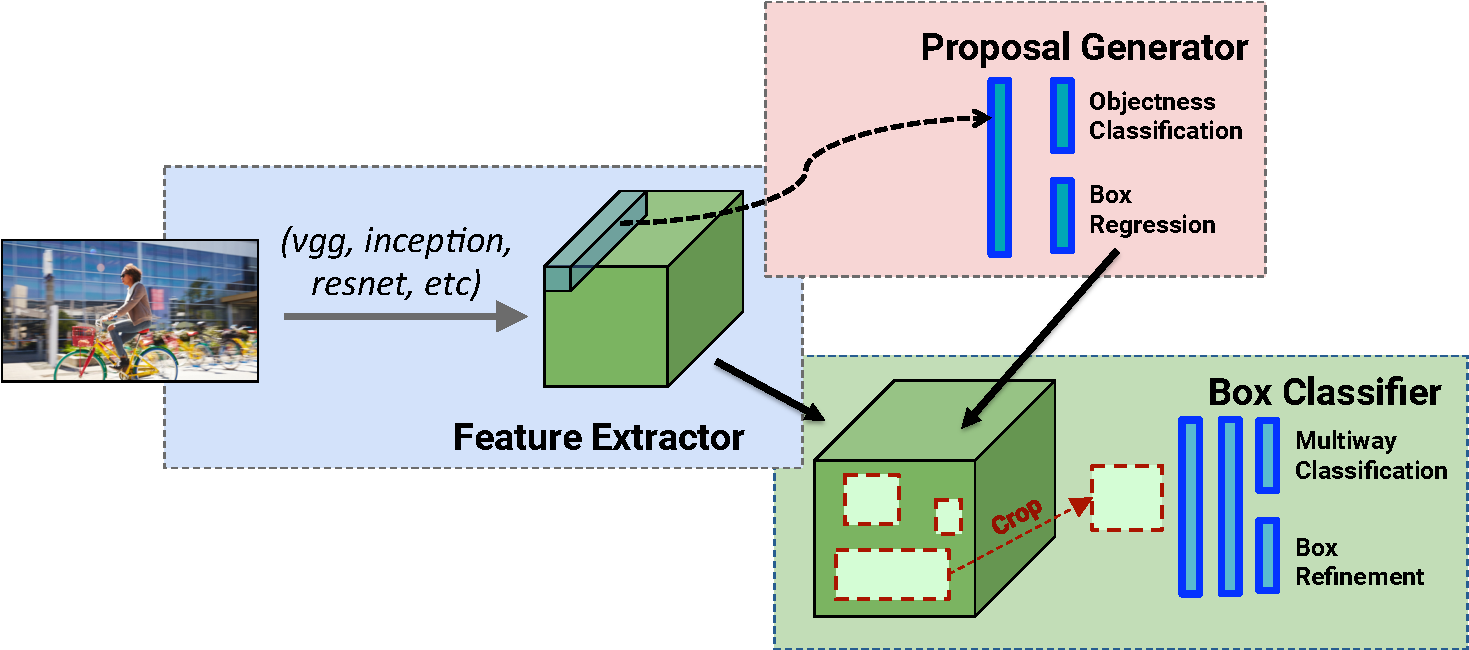
\includegraphics[width=0.85\linewidth]{fasterrcnn_diagram.pdf}
		\caption[The \FRCNN{} architecture]{The \FRCNN{} architecture \citep[credit to][]{detection_benchmark}
		\label{fig:faster_rcnn}
		}
	\end{figure}

	The task of object detection builds upon that of image classification since architectures based on region proposals (see \autoref{sec:related_detection}) can be seen as a two stage algorithm: the first part extracts possible object bounding boxes as a sub-image of the input, while the second one predicts the class associated with each candidate. It is of no surprise then that object detection greatly benefits from the super-human accuracy of deep neural networks \citep{superhuman_classif}. We chose to pair the \FRCNN{} detection architecture with the \RESNET{} feature extractor \citep{resnet}, since this has been proved to give a good trade-off between speed and detection accuracy on the standard challenge of ILSCVR \citep{detection_benchmark}. In what follows we present the main building blocks of this architecture.

	%----------------------------------------------------------------------------------------

	\subsection{Feature extraction}\label{sec:resnet}
		In order to perform detection on an input image, we first need to extract representative high-level features from the raw pixel values. To this end, we employ the \RESNET{} convolutional architecture which has won many competitions in classification, detection and segmentation.

		The novelty of this approach relies in forcing the network to learn a \emph{residual} mapping \(\mathcal{F}(\ve{x}) := \mathcal{H}(\ve{x}) - \ve{x}\), where \(\mathcal{H}(\ve{x})\) represents a desired mapping from input \(\ve{x}\), which is to be fit through a few stacked layers (\autoref{fig:resnet} left). This comes from the observation that the optimal function to be learnt could be closer to the identity mapping than to a zero mapping. Therefore, the new formulation eases the job of the optimiser since it only has to find perturbations around the identity mapping, rather than learn a completely new function.
		% http://www.robots.ox.ac.uk/~vgg/publications/2015/Jaderberg15b/jaderberg15b.pdf gives a good started about many things, including how ConvNets work

		Moreover, in order to keep the number of parameters as small as possible and have reasonable training times for very deep architectures (101 layers), standard convolutions are replaced by bottleneck-blocks of convolutions (\autoref{fig:resnet} right). Such blocks are formed by concatenating a \(1 \times 1\) convolutional layer at each end of the \(3 \times 3\) layer. The ``prefix'' layer reduces the number of filters while the ``suffix'' one increases it back, thus reducing the computational cost of the heavier middle layer.

		\begin{figure}
			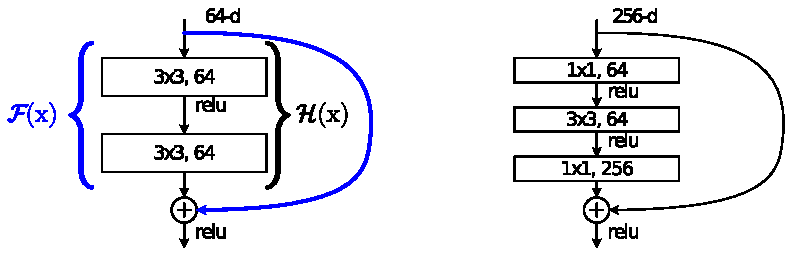
\includegraphics[width=0.85\linewidth]{resnet_blue}
			\caption[ResNet blocks]{
				The left part represents a normal ResNet block which forces the network to learn the residual mapping \(\mathcal{F}(\ve{x}) := \mathcal{H}(\ve{x}) - \ve{x}\) through the skip connection shown in blue. The right part shows a ``bottleneck'' block used in \RESNET{}.

				\raggedleft{\citep[credit to][]{resnet}}
				\label{fig:resnet}
			}
		\end{figure}

	%----------------------------------------------------------------------------------------

	\subsection{Region proposal network}\label{sec:frcnn_rpn}
		In order to bring the inference speed closer to real-time, \FRCNN{} improves on the bottleneck of previous approaches, namely the proposal of object candidates. Instead of relying on highly-engineered low-level features of super-pixels, the architecture reuses the convolutional feature map generated for the region classification step.

		This is achieved through another small, fully-convolutional network which is slid along the final layer of the feature map. The window at each location is projected into a lower dimensional feature that is used to predict \(k\) region bounds as well as \(k\) ``objectness'' scores. Each predicted region \(k_i\) is encoded as 4 coordinates \(\ve{t}_i = (x, y, w, h)_i\) that define the bounding box \emph{relative} to a set of predefined boxes called \emph{anchors}. This mechanism allows the detection of multiple scales and aspect ratios in one pass through the network, thus avoiding the need of image pyramids and further reducing the computational cost.

		For training the RPN, the following loss function has to be minimised:
		\begin{equation*}\label{eq:rpn_loss}
		L(\ve{p}_i, \ve{t}_i) =
			\frac{1}{N_{\cls}}\sum_i L_{\cls}(\ve{p}_i, \ve{p}^{*}_i)
			+ \lambda\frac{1}{N_{\reg}}\sum_i  \ve{p}^{*}_i L_{\reg}(\ve{t}_i, \ve{t}^{*}_i);
		\end{equation*}
		\(\ve{p}_i\) represents the probability that anchor \(i\) is an object; \(\ve{p}^{*}_i\) is the label of this anchor (\(1\) when it significantly overlaps a ground truth box) and \(\ve{t}_i, \ve{t}^{*}_i\) encode the anchor's and ground truth's coordinates, respectively.

		The loss jointly minimised  the ``objectness'' classification term \(L_{\cls}\) for an anchor \(i\) in the minibatch and the bounding box regression term \(L_{\reg}\); the two are balanced by the hyper-parameter \(\lambda\). The regression term is only taken into account for positive anchors (\(p^{*}_i = 1\)), which are those overlapping a ground truth box with an Intersection-over-Union (\(\iou\)) ratio above threshold \(\tau_+ = 0.7\).

	%----------------------------------------------------------------------------------------

	\subsection{Training}\label{sec:frcnn_train}
		In addition to generating object candidates with the RPN, the \FRCNN{} architecture also needs to classify the generated proposals. For this, it uses the Fast R-CNN architecture and trains both of them at the same time, as shown in \autoref{fig:faster_rcnn}. The forward pass generates box proposals that the classifier considers to be fixed for its training. This easy implementation ignores the gradients with regards to the coordinates of the proposal boxes, so it is only an approximation of the joint training procedure. However, its results are close to those obtained by alternating the training of the two networks, while being significantly faster.

		Instead of training the whole architecture from scratch, we gain significant time by using transfer learning and starting with a model that performs well on the ImageNet challenge. We replace its final softmax layer so that it only predicts among our two classes of interest: \texttt{text} or \texttt{background}.

		We hypothesize that the object / not-object distinction is easier to make for text on white background documents than it is for an ImageNet object in the wild. Therefore, we set hyperparameter \(\lambda = 2\) in order to give preference to the box regression loss. Moreover, in order to account for text's wide aspect ratio and relatively constant height in our documents, we change the default anchors to be similarly wide (ratios \(\{2, 4, 6, 8, 10\}\)) and with a limited set of scales (heights of \(\{50, 75, 100\}\)px). This further helps the box regression part to converge.

		We use the stochastic gradient descent (SGD) optimiser with momentum which updates the weights \(\ve{W}\) of the network using an exponential moving average of the gradients:\[
		\begin{split}
			\ve{V}_t &= \beta \ve{V}_{t-1} + (1-\beta) \nabla_w L (\ve{W}, \ve{X}, \ve{y}),\\
			\ve{W} &= \ve{W} - \alpha \ve{V}_t,
		\end{split}
		\]
		where \(\alpha\) is the learning rate and \(\beta\) is the momentum value. We use \(\beta = 0.9\) and a step decay schedule for the learning rate \[
			\alpha = \alpha_0 * 0.3 ^ {\floor{\frac{\mathit{step}}{1000}}},
		\]
		which starts with the initial learning rate \(\alpha_0 = 0.003\) and decreases it every 1000 steps.

		We feed the network one image at a time, resized such that its shorter side is 600px wide. Note, however, that a minibatch is formed of bounding boxes, so many candidates can be generated from a single input image and a set of anchors. Several hyper-parameters control the composition of the batches:
		\begin{description}
			\item[number of proposals (\(\mathit{value} = 300\))] How many object proposals are generated in each batch.

			\item[positive to negative ratio (\(\mathit{value} = 0.5\))] For a robust classification and convergence of ``objectness'' score, it is important that examples of both positive and negative candidates are generated.

			\item[positive IoU threshold (\(\tau_{+} = 0.7\))] An anchor is considered positive when \(\mathit{overlap}(\mathit{anchor}, \mathit{truthBox}) > \tau_+\). While \(0.7\) could be considered low for text objects (see \autoref{fig:text_overlap_example}), setting this value too high in the early stages leads to a lower number of positive candidate and slows down convergence of \(L_{cls}\).

			\item[negative IoU threshold (\(\tau_{-} = 0.3\))] Similar to \(\tau_{+}\), but for marking candidates as negative examples.

			\item[NMS confidence threshold (\(\mathit{value} = 0.0\))] When a candidate has a low confidence score, we can suppress it from contributing to the loss. We effectively disable this filter because we want to force the network to give high-confidence predictions, therefore it should learn from all examples.

			\item[NMS IoU threshold (\(\tau_{\textsc{nms}} = 0.7\))] When several proposals overlap each other, we should keep only one of them in the batch in order to increase proposal's diversity. This parameter controls when we can consider that a proposal is redundant to another one, in terms of their overlap.

		\end{description}

		On every experiment we monitor the training progress by intermittently evaluating the model on a validation dataset of images from the same category. The training is stopped once there is no significant improvement for more than two epochs, despite a decreasing learning rate.


%========================================================================================

\section{Connectionist Text Proposal Network}\label{sec:ctpn}
	% http://i.cs.hku.hk/~kykwong/publications/wliu_bmvc16.pdf This has a good simple explanation of ResNet and LSTM and what-not

	Once we established the feasibility of object detection techniques for our task via \FRCNN{}, we searched for improvements that could increase the quality of the detections. The rest of the section presents an extension to the previous architecture based on the work of \citet{CRNN} which is designed specifically for text detection.

	%----------------------------------------------------------------------------------------

	\subsection{RPN becomes CTPN}
		The main novelty of \FRCNN{} consisted of generating object candidates with a fast additional network based on a set of anchors which are combined in different scales and aspect ratios. This work builds on the observation that text does not have a closed boundary since it is composed of a sequence of letters and strokes. As such, a text ``object'' can have arbitrary width, which is difficult to accommodate with the standard anchor mechanism. The algorithm would need anchors of many different aspect ratios and even so, it would still be difficult to completely detect a line that is much longer than any of the ones in the training set.

		The \CTPN{} architecture proposes an ingenious solution: break down text objects into a series of adjacent boxes of constant-width and similar height; consequently, learn to predict a series of anchors that respect the same constraints, called \emph{fine-scale} proposals (\autoref{fig:ctpn_splitting}). Therefore, now the box regression is only concerned with the anchor's height \(h\), since the width is fixed and the RPN only has to learn text-specific features of a reduced bounding box of size \(h \times 16\).

		While the above is a clever twist on the original RPN, the merging of fine-scale proposals requires high-confidence outputs for all candidates in a series, i.e. for all boxes on the same line; otherwise it easily results in a segmented prediction. This is problematic especially when we want to detect multiple words as a single sequence on a line (\autoref{fig:ctpn_merging}), since each box is judged independently, based on its contents. As a solution, the series aspect should be exploited, and box prediction should make use of the context. To this end, the text proposal network is enhanced with a bi-directional LSTM layer
			\footnote{We will detail the inner workings of a similar LSTM layer in \autoref{sec:LSTM}}
		that sits of top of the sliding window network and propagates context between multiple predictions (\autoref{fig:ctpn_arch}). In this way, the network provides more consistency both for the confidence and for the heights of the boxes.

		A final refinement mentioned in the original paper consists of a regression of side margins of the first and last anchors on a detected line. Since we achieved good results without this part, we postponed its implementation for future improvements. As such, the loss function becomes almost identical to the RPN loss:
		\begin{equation*}\label{eq:ctpn_loss}
		L(\ve{p}_i, \ve{v}_i) =
			\frac{1}{N_{\cls}}\sum_i L_{\cls}(\ve{p}_i, \ve{p}^{*}_i)
			+ \lambda\frac{1}{N_{\reg}}\sum_j L_{\reg}(\ve{v}_j, \ve{v}^{*}_j),
		\end{equation*}
		except for the regression loss \(L_{\reg}\) which now only regresses a pair of coordinates, the centre and the height \(\ve{v}_j = \{v_c, v_h\}\) of the \(j\)-th anchor from the predefined set.


		\begin{figure}
			\begin{subfigure}[c]{.69\linewidth}
				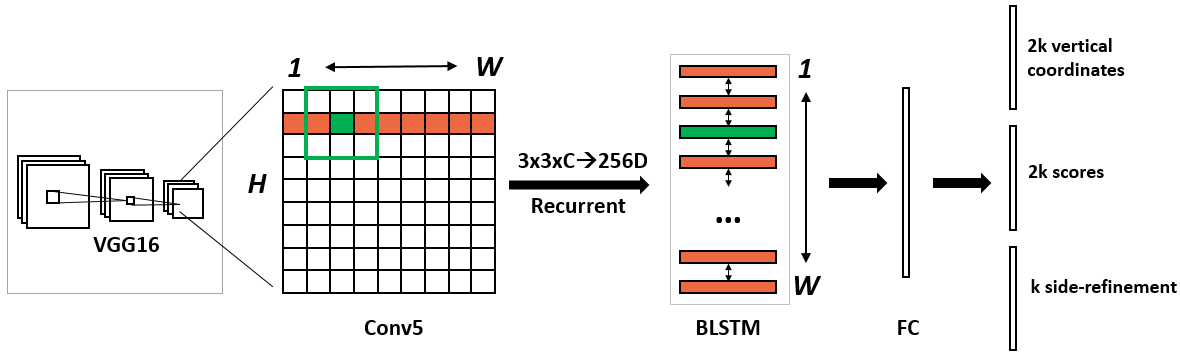
\includegraphics{ctpn_architecture}
				\caption{Overview \citep{ctpn}}\label{fig:ctpn_arch}
			\end{subfigure}
			\begin{subfigure}[c]{.30\linewidth}
				\begin{subfigure}{\linewidth}
					
\includegraphics{ctpn_orig}
					
\includegraphics{ctpn_split}
					\caption{Box splitting}\label{fig:ctpn_splitting}
				\end{subfigure}
				\par\bigskip
				\begin{subfigure}{\linewidth}
					
\includegraphics{ctpn_recon_fine}
					
\includegraphics{ctpn_recon_merged}
					\caption{Box merging}\label{fig:ctpn_merging}
				\end{subfigure}
			\end{subfigure}
			\caption[The \CTPN{} architecture]{The Connectionist Text Proposal Network:

			\subref{fig:ctpn_arch} The architecture comprises of the VGG feature extractor, succeeded by a fully-convolutional network coupled with an LSTM for fine-scale proposals.

 			\subref{fig:ctpn_splitting} Original bounding box and the corresponding series of equal width boxes.

 			\subref{fig:ctpn_merging} Predicted fine-scale proposals and the resulting bounding boxes. Note the limited merging due to missing proposals.
			}
		\end{figure}

	%----------------------------------------------------------------------------------------

	\subsection{Training}
		The original paper does not mention how fine-scale proposals are generated from the original bounding boxes, nor how they are merged to predict a large box. We found this to be an important implementation detail as it introduces a hyper-parameter \(\tau_{gap}\) which is a threshold for the maximum gap allowed between two neighbouring proposals. For example, in \autoref{fig:ctpn_merging} a small \(\tau_{gap}\) resulted in an overly-segmented of a word, whereas a too large \(\tau_{gap}\) would have merged the words together. Whether this is desired or not depends on the context. We have set \(\tau_{gap} = 24\)px, which is \(1.5\) times larger than the anchor width.

		Once the \CTPN{} predicts fine-scale proposals, these are classified into \texttt{text} or \texttt{back\-ground} by the same Fast R-CNN core as before. However, in this case we use a different feature extractor, namely the VGG network \citep{VGG}, in order to reproduce the setup of the original work. As in the previous case, we do not train from scratch but instead we start with the weights provided by the authors, who used 3000 images of text in the wild.

		We observed that a large number of the generated anchors were meaningless in our context due to little variation of text height. Therefore, we changed the default set of anchors to use only 3 different heights: \(\{10, 16, 23\}\) pixels which correspond to the most common ground truth heights after resizing the image to be 600px wide. This reduced the iteration time more than three times and also resulted in faster convergence of the training.

		We minimised the loss function using the Adam optimiser \citep{adam}, with an initial learning rate \(\lambda = 0.0001\). Furthermore, we used \(L_2\) regulariser with balancing weight \(\lambda_{L2} = 0.0005\).

%========================================================================================


\section{Datasets and experiments}\label{sec:detection_experiments}
	%-- INTRO -------------------------------------------------------------------------------
		Given the large number of parameters in deep neural networks (\(\approx 6 \times 10^8\) for \RESNET{}), it is clear that large amounts of training data are needed to train our architectures. Since this is lacking for our project, we must find alternative sources of handwritten text, ideally in the same language as the documents, i.e. French. Moreover, as was noted in \autoref{sec:challenges}, our documents have a difficult, albeit well-defined format, and less than optimal quality.

		The RIMES database \citep{rimes} is the result of a huge data collection effort by the French ministries of defense and research, which was set up in order to create a new, consistent database of handwritten text. Its novelty was that it also included mixed pages, with handwritten and printed text, as well as being almost completely unconstrained with regards to the content of the text.	It contains more than \(50\,000\) handwritten words that are made available individually, or in lines (more than \(9000\)), or in paragraphs (more than \(1500\)). We will base most of our experiments on this collection of handwritten text, though the following sections will detail different ways of adapting it to our use case. Additionally, we will also use our handwriting generator from \autoref{sec:generator} to analyse the influence of the training set and to overcome limitations of the RIMES database.

	%----------------------------------------------------------------------------------------

	\subsection{Evaluation framework}\label{sec:detection_eval}
		Before delving deeper into the details of our experiments, it is necessary to introduce requirements of the task and measures for quantifying their achievement. This section introduces one such measure that we will use for quickly assessing the outcome of an experiment. An in-depth evaluation will be carried on in \autoref{sec:detection_results}.

		Judging a detection result via a single number is a very difficult task, since the lack of a \emph{cost} associated with a false positive requires a trade-off between different types of errors. Standard object detection challenges such as PASCAL VOC \citep{pascal_voc} required participants to rank their results by a score, commonly referred to as \emph{confidence}. This allows the evaluation of a trade-off between false positives and false negatives by assessing the area under the precision/recall curve. To this end, the Average Precision is used:\[
			\operatorname{AP} = \frac{1}{11} \sum_{r \in [0,1]} p(r),
		\] which is the mean of precisions \(p\) computed at eleven equally spaced recall values \(r \in [0,1]\).

		Two essential observations need to be made. First, a great importance is given to the confidence score, since recall and precision are defined by only considering examples ranked above a given rank. Second, the measure does \emph{not} define what a positive result means. For object detection, a predicted bounding box \(B^p\) is positively mapped to \mbox{ground truth} box \(B^{gt}\) when their overlap exceeds a given threshold \(\tau\). The overlap is defined as \[
			\iou(B^p, B^{gt}) = \frac{\mathit{area}(B^p \cap B^{gt})}{\mathit{area}(B^p \cup B^{gt})}.
		\] In general, the threshold is set at \(\tau = 0.5\) and the measure is denoted by \(\AP\).

		Since text detection is a particular case of object detection, it generally subscribes to the same evaluation criteria. However, text is more than a simple object with binary presence; it consists of a sequence of characters, all of which are mandatory and of \emph{equal} importance to the meaning. This is in contrast to objects in general images such as those in the PASCAL VOC database. While such objects also admit a hierarchical structure (e.g.\ a cat has eyes, ears, legs, tail etc.), the presence of their sub-elements is not always mandatory; on the contrary, a subset of composing elements is almost always hidden due to self occlusions. This allows some partial detections to be considered valid in the context of objects (see \autoref{fig:cindy}). Text detection cannot afford such flexibility, since we aim to use the detections in a subsequent step of transcription. This requires that bounding boxes include all relevant text and, ideally, no other text fragments such as parts of the line above or below (see \autoref{fig:text_overlap_example}).

		Considering that in our documents text lines are close to each other, we demand the detections to be as tight as possible around the text. However, given the lack of a baseline in such challenging documents, we will base our intermediate decisions on the standard measure of \(\AP\). This allows us to compare our text detection models with their object detection counterparts.

		\subsubsection*{Test data}\label{sec:detection_test_data}

		Given that our approaches rely on transferring knowledge from generated data, we need an objective way of comparing their performance. To this end, we constructed a \ds{Test} dataset to provide ground truth labels on real-world data. This consists of 26 annotated statements which amount to approximately 1400 bounding boxes.

		\begin{figure}
			\begin{subfigure}[b]{0.49\linewidth}
				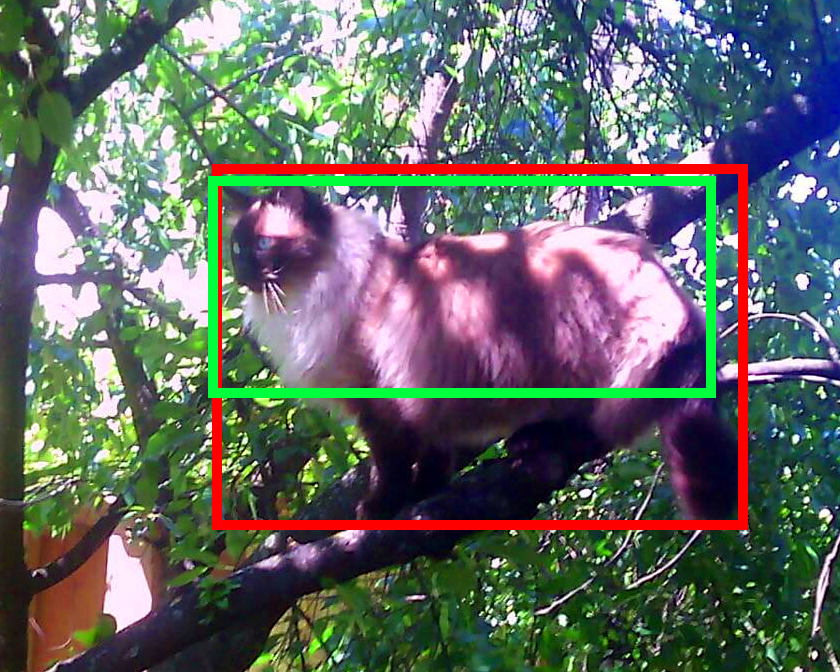
\includegraphics{cindy}
				\caption{\label{fig:cindy}}
			\end{subfigure}
			\begin{subfigure}[b]{0.49\linewidth}
				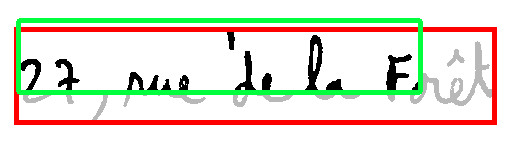
\includegraphics{text_iou}
				\vspace{2em} % no idea why this works. it was supposed to add space *between* the images, but oh well...
				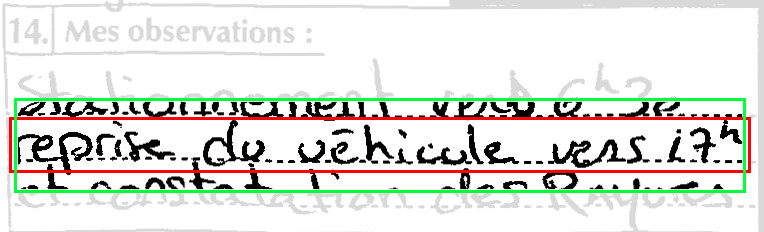
\includegraphics{text2_iou}
				\caption{\label{fig:text_overlap_example}}
			\end{subfigure}
			\caption[Overlap examples]{Overlap examples: red shows ground truth; green shows detection. In all cases \(\iou = 0.55\). While this is a valid detection threshold for a normal object, it is unsatisfactory for text recognition.
			}
			\label{fig:overlap_example}
		\end{figure}

	%----------------------------------------------------------------------------------------

	\subsection{Collage of paragraphs}
		\subsubsection*{\ds{Collage} dataset}

			For the first training session, we used images of paragraphs from the database along with their segmentation into lines as labels. To make them resemble the format of the documents, we juxtaposed two or three paragraphs picked at random from the database. These were corrected for rotation and augmented with borders to look similar to the sections of a document (\autoref{fig:collage}). We generated \(3500\) examples for training and \(500\) for validation.

		%........................................................................................

		\subsubsection*{Outcome}

			A \FRCNN{} model trained on this dataset converged rather quickly, in \(\approx 8000\) iterations. On its validation data, the model achieves a remarkably high performance, with \mbox{\(\AP = 0.96\)}. Note that the best performance of any model in object detection so far is \(\AP \simeq 0.73\), which clearly indicates that the task is very easy for the chosen model. However, the performance does not extend to the \ds{Test} dataset, achieving only \(\AP = 0.02\). This highlights the differences between the training and the test datasets. The most likely cause of the performance drop is the presence of additional elements in a real document, such as printed text and indicator lines, which do not exist in the training images. Therefore, the negative anchors generated by the algorithm are inevitably white boxes. In addition, the model regresses the anchor sizes to predict boxes of shape similar to the input lines. These display little variation in width and are, in general, much wider than the text fields of a document.

		\begin{figure}
			\begin{subfigure}[c]{\textwidth}
				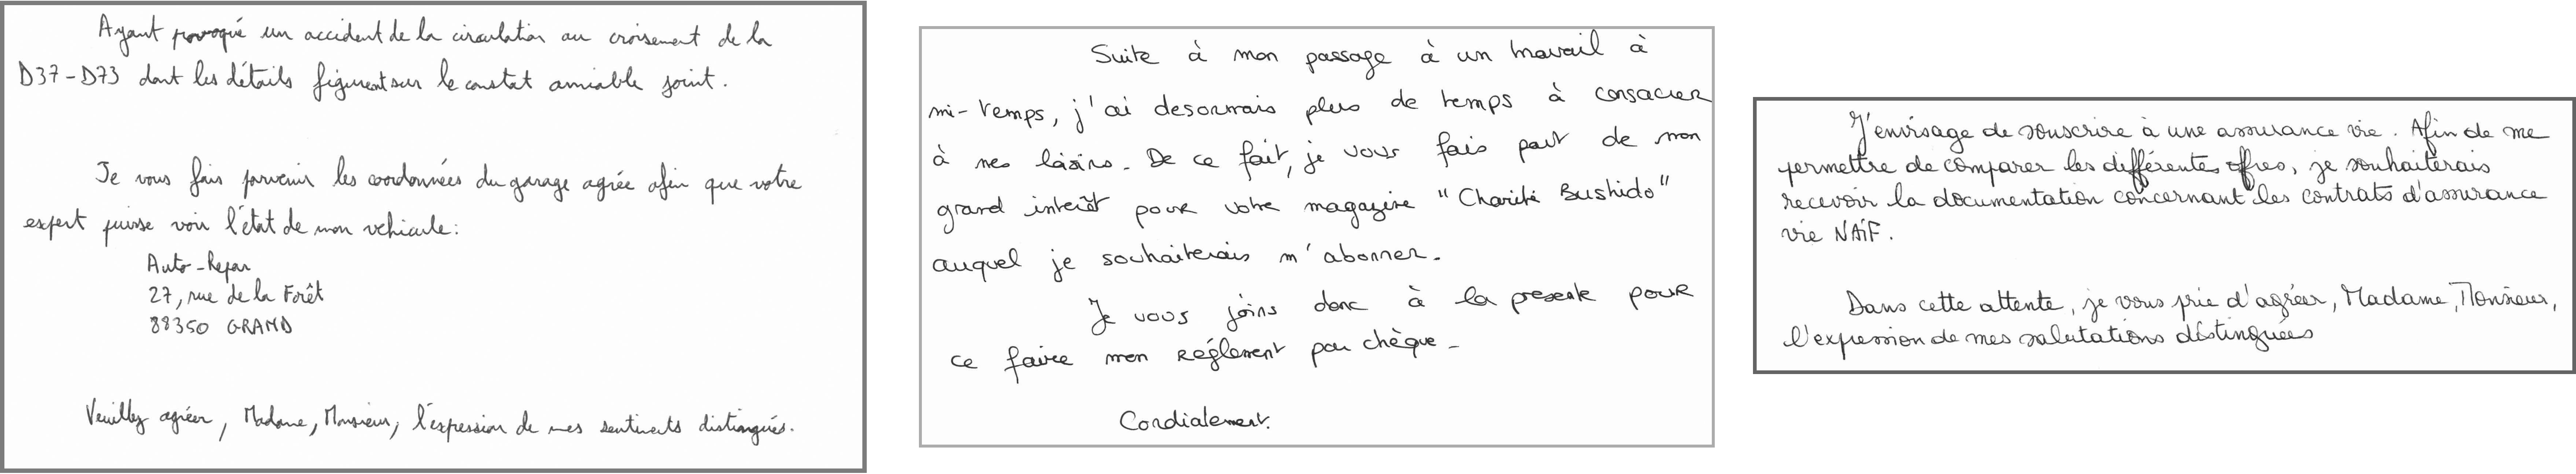
\includegraphics{collage_3}
				\caption{}
				\label{sfig:collage_clean}
			\end{subfigure}
			\vspace{1em}

			\begin{subfigure}[c]{\textwidth}
				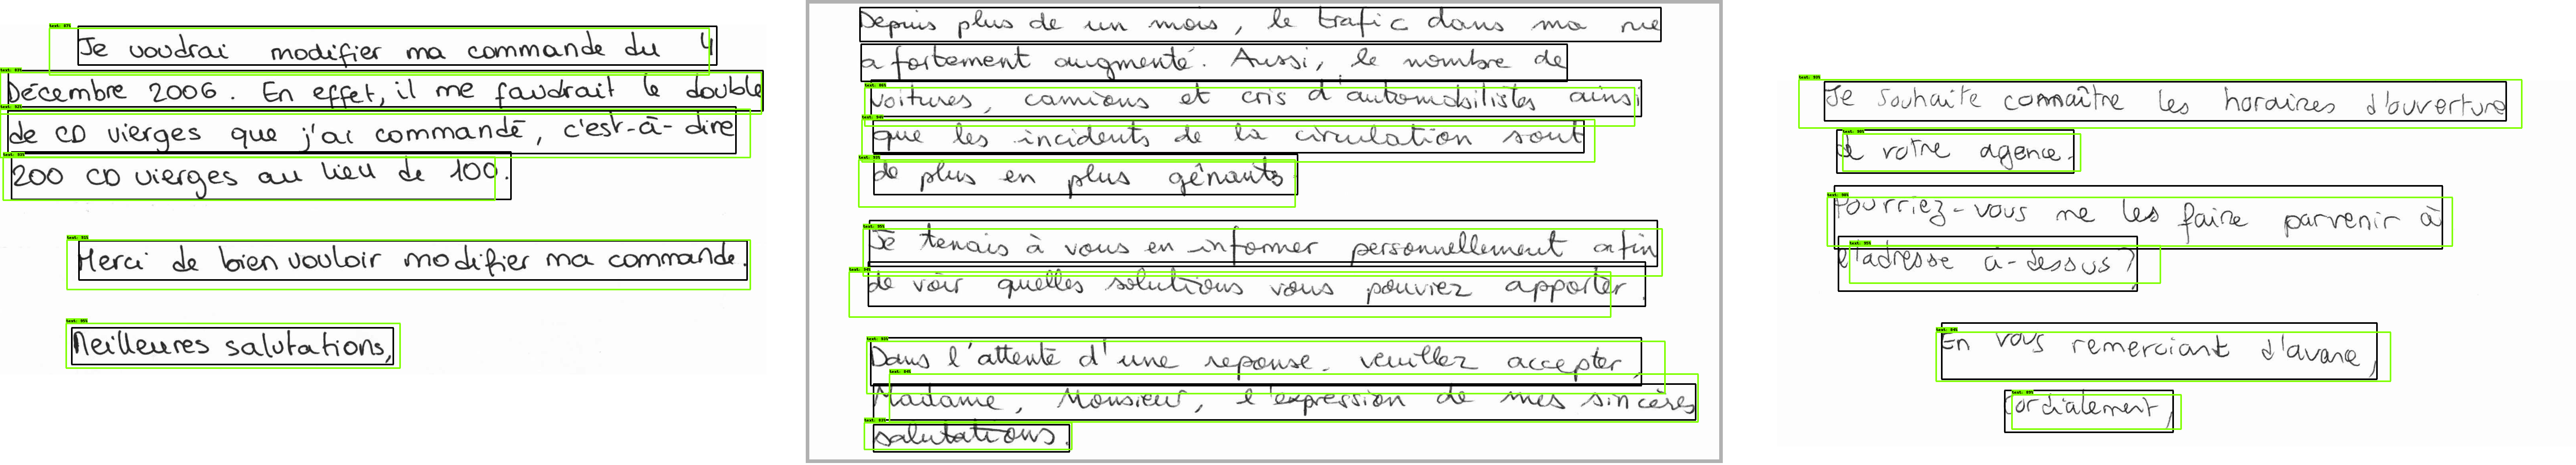
\includegraphics{collage_3_detected}
				\caption{}
				\label{sfig:collage_detect}
			\end{subfigure}
			\caption[\ds{Collage} dataset]{
				The \ds{Collage} dataset.
				\subref{sfig:collage_clean}: Example of generated collage document with 3 juxtaposed paragraphs.
				\subref{sfig:collage_detect}: The detection performed on such a document, with ground truth in black and detection result in green.
			}
			\label{fig:collage}
		\end{figure}

	%----------------------------------------------------------------------------------------

	\subsection{RIMES-filled templates}
		%........................................................................................
		% subsubsection: general description

			To address the limitations of the \ds{Collage} dataset and allow the model to learn more complex patterns, we propose to generate images which resemble more the real documents. To this end, we fill accident statement templates of 4 different styles with handwritten text from a database. This results in realistic looking documents while saving the high cost of manual labelling.

		%........................................................................................

		\subsubsection*{\ds{Template} and \ds{Template_bin} datasets}\label{sec:rimes_template}
			A template is formed by adding input placeholders to an empty document (\autoref{fig:template}). These correspond to the standard places that the users need to fill as well as non-standard places where users regularly add information. To increase the variation of the data, only a subset of the placeholders are filled on each template instance and the input text is shifted horizontally inside the placeholder by a random amount. We investigate two possible text sources for filling the templates.

			\begin{figure}
				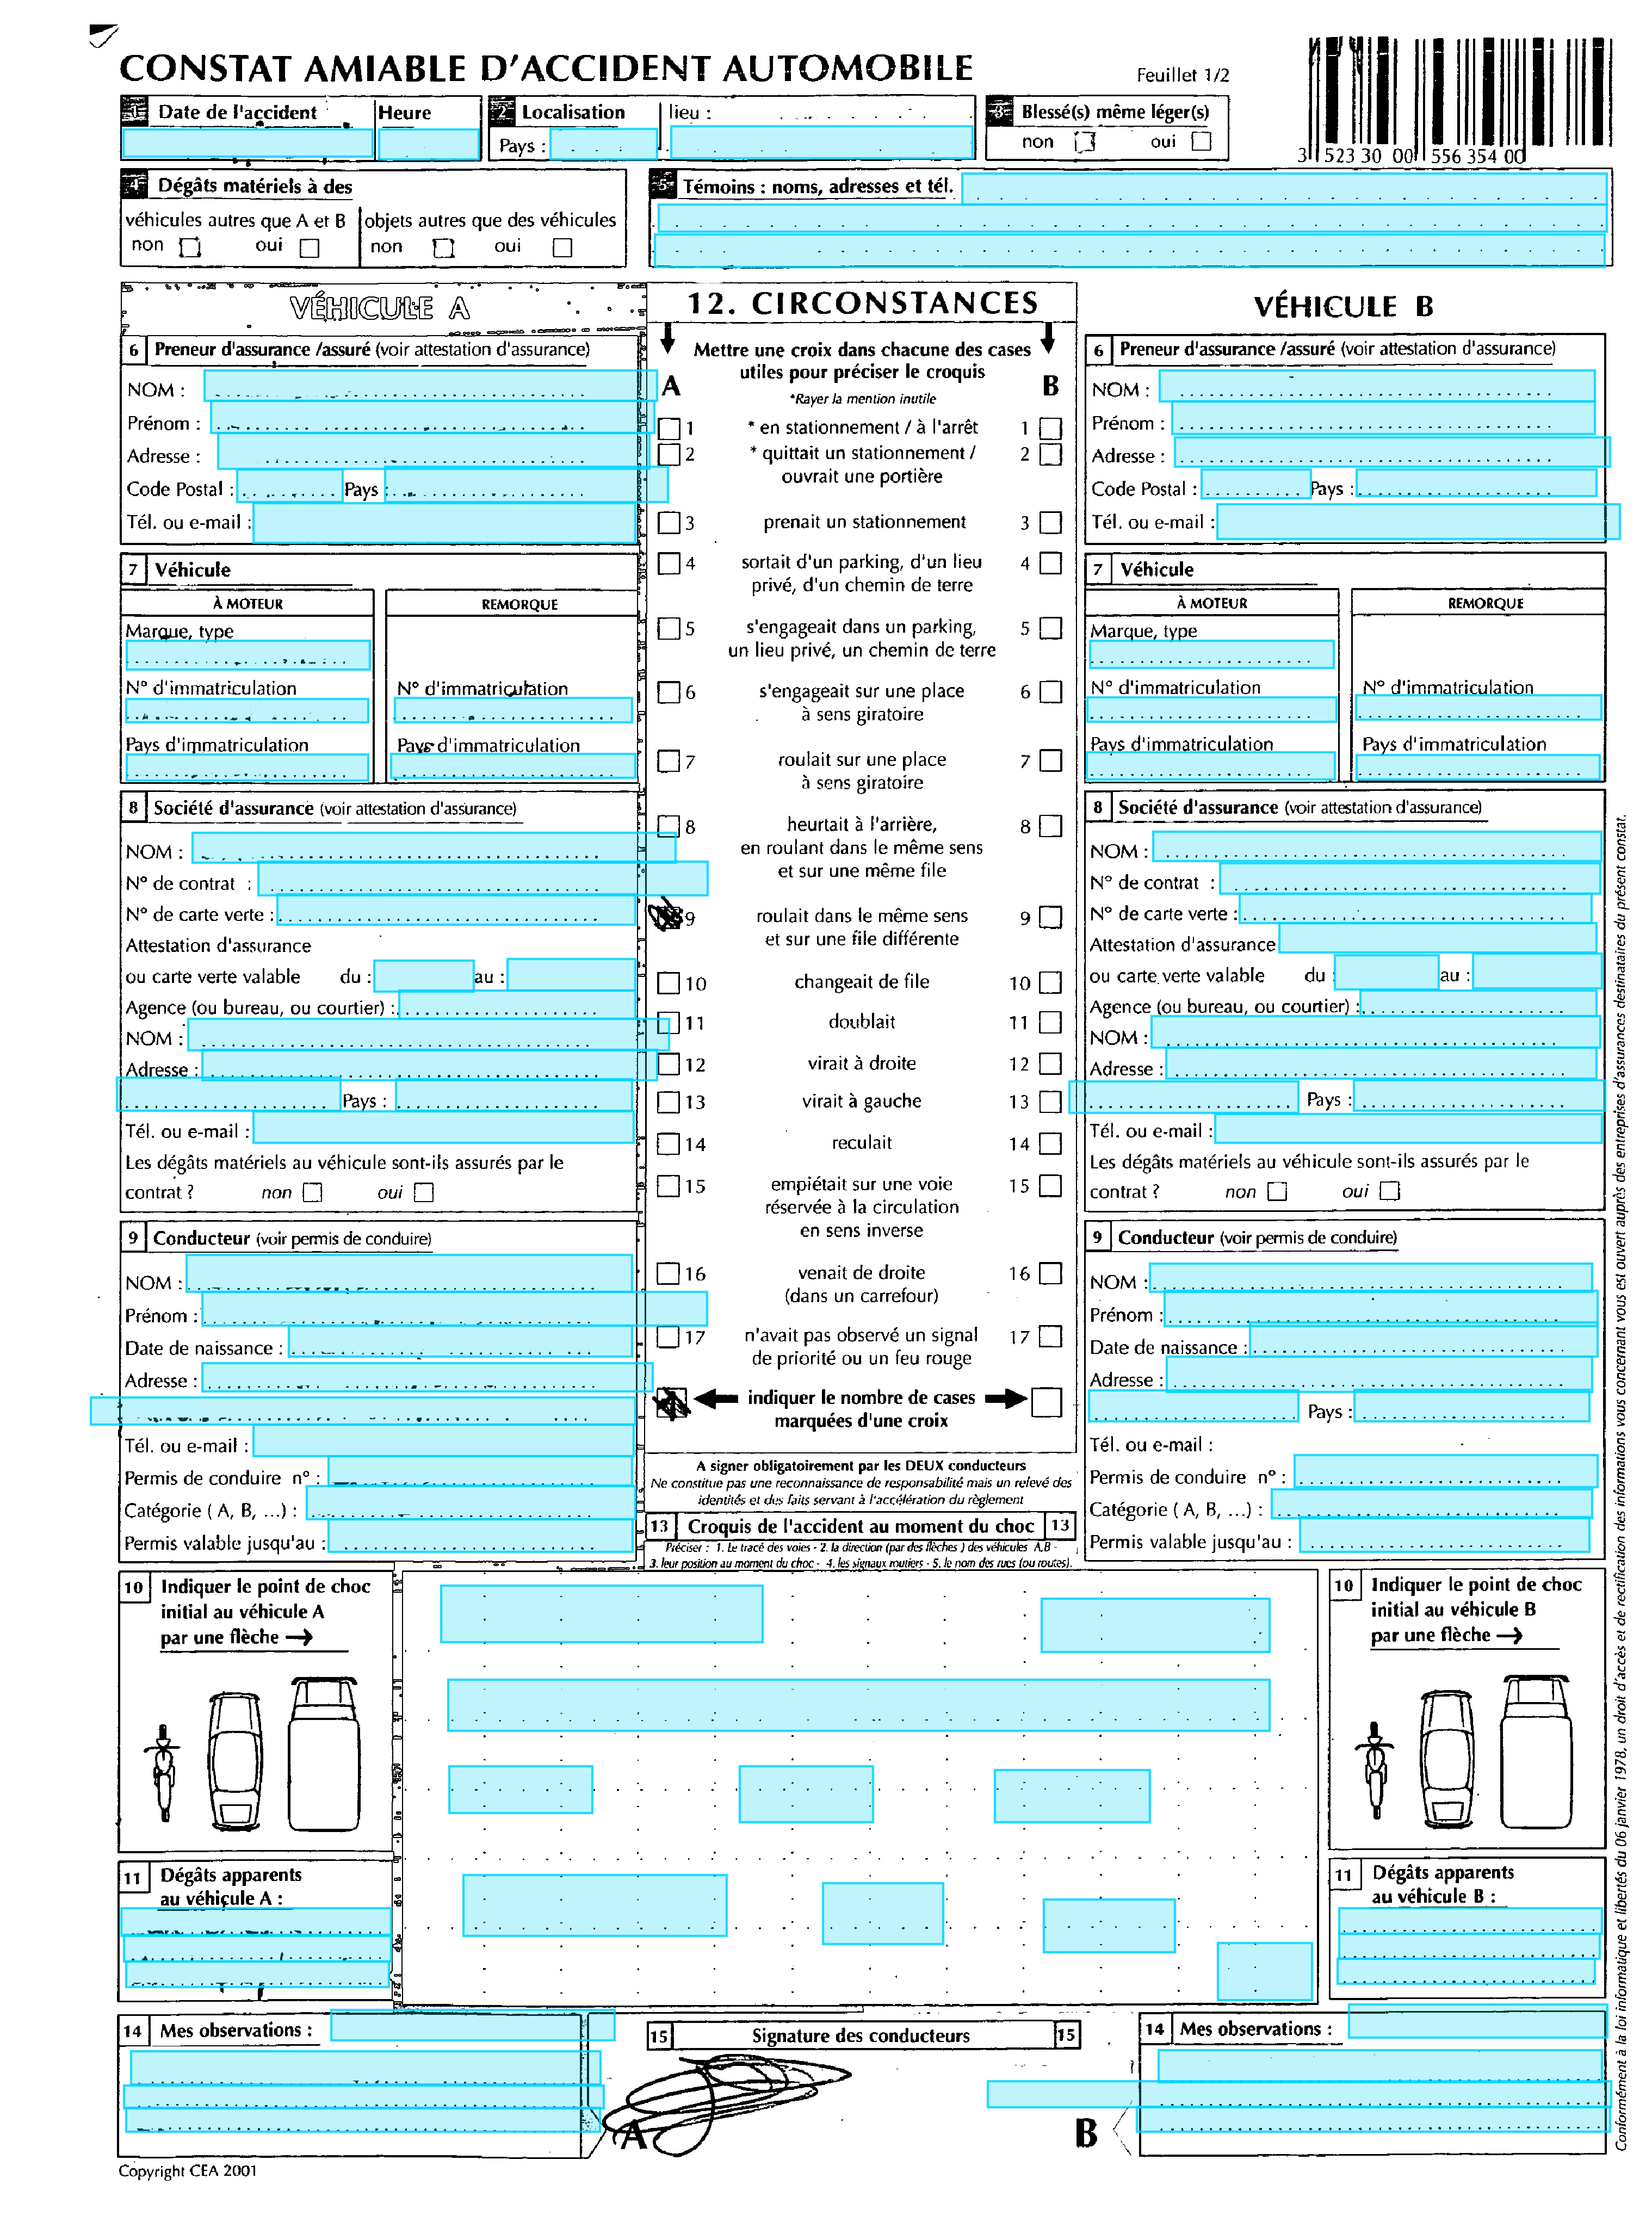
\includegraphics{template_empty}
				\caption[Document template]{An empty document template. Note that the placeholders are slightly bigger than the location for text entry in order to allow text that goes out of bounds. Also, there are placeholders in places that do not correspond to any field, which matches how people use these documents.}
				\label{fig:template}
			\end{figure}


			The first one consists of images of \emph{individual} words from the RIMES database. This has the advantage of tight bounding boxes around the text, which we established as an important criterion in \autoref{sec:detection_eval}. Also, it allows us to keep the ground truth text associated with each box, which will also make them useful for the transcription step. On the other hand, this source also poses some problems. First, words are generally shorter than the placeholders, so we would need to concatenate several words to resemble the real data. Since the word order was lost when constructing the database, this has the disadvantage that lines formed in this way do not follow any sentence structure. Furthermore, words with ascenders and descenders would need to be aligned to their baseline, which is especially difficult to estimate for short words. Finally, handwriting styles from multiple authors would be combined on the same line and in the same document section.

			The second source of text consists of images of text lines from the same database. This addresses the problems of word concatenation, but introduces another difficulty: the lines are usually longer than the placeholders, so they need to be cut. However, thinking forward about the text transcription part, we immediately realise that in order to have reliable \((\mathtt{image}, \mathtt{label})\) pairs, we must ensure line images are split \emph{only between the words}. We use the following algorithm to detect good splitting points in image \(\ve{I}\): % https://tex.stackexchange.com/questions/172399/how-to-write-sentences-in-an-algorithm-in-latex https://tex.stackexchange.com/questions/142922/how-to-align-text-within-an-algorithm-environment
			\noindent\begin{minipage}{\linewidth}
			\begin{enumerate}
				\item use the line transcription labels to find the number of words \(n\)
				\item project the image columns horizontally, accumulating their sum into \[
					\ve{p}_c = \sum_{r = 1..H }\ve{I}_{r,c}
				\]
				\item find the continuous runs of zero \(\ve{z} = \{ (i, j) \mid \ve{p}_k = 0, \forall k \in [i, j] \}\); these correspond to gaps between letters (marked in red in \autoref{fig:baseline_ok})
				\item take \(n\) widest gaps \(\ve{z}'\) from \(\ve{z}\), where the gap width \(w := j - i\)
				\item split at columns \(c_k = \frac{j_k - i_k}{2}, \forall (i_k, j_k) \in \ve{z}'\).
			\end{enumerate}
			\end{minipage}
			\\

			To avoid placeholders filled with very short words, we add multiple words to the same placeholder until it is at least 70\% filled. Note that unlike the first text source, these words come in order from the original line, split by the above algorithm. Moreover, lines come sequentially from the same paragraph, so there is writer consistency for a good part of a template, just like in the real world.

		%........................................................................................

		\subsubsection*{Baseline detection}
			When humans fill a statement template, the baseline of their handwriting lies roughly on an indicated line.  We purposely set the placeholder's bottom edge on this line in the interest of aligning the text image in a similar manner. Then we use the following simple procedure to find the baseline row \(r_b\) of a text image \(\ve{I}\) of size \(H \times W\) (\autoref{fig:baseline}):
			\noindent\begin{minipage}{\linewidth}
			\begin{enumerate}
				\item project the rows of the image by averaging the pixel values: \[
					\ve{p}_r = \frac{1}{W} \sum_c I_{r,c}
				\]
				\item let \(m = \operatorname{median}(\ve{p})\)
				\item the baseline is the first row \(r_b\) where \(\ve{p}_{r_b} > m\), \(b = H..1\).
			\end{enumerate}
			\end{minipage}\\

			The method above works well as long as a few assumptions hold. First, the text image has to be horizontal. In case it is not (see \autoref{fig:baseline_skewed}), we de-skew it by rotating with the average angle of Hough lines. Second, the input line has to be correctly segmented vertically. As a counter example, \autoref{fig:baseline_segmentation} shows that due to another text line present in the same image it is difficult to segment the words correctly. Fortunately, the database does not contain many examples that break these assumptions and we can reject tokens resulted from a failed segmentation based on their length.

			\begin{figure}
				\begin{subfigure}{\linewidth}
					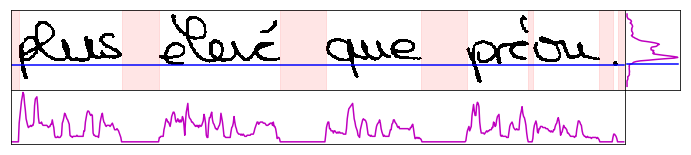
\includegraphics{baseline_ok}
					\caption{Good and clean horizontal image}
					\label{fig:baseline_ok}
				\end{subfigure}
				\bigskip

				\begin{subfigure}{\linewidth}
					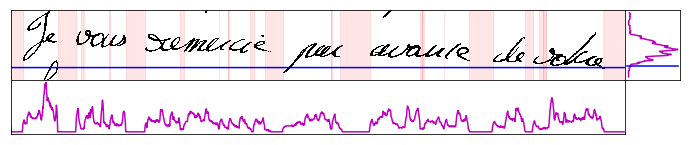
\includegraphics{baseline_skewed}
					\caption{Skewed image}
					\label{fig:baseline_skewed}
				\end{subfigure}
				\bigskip

				\begin{subfigure}{\linewidth}
					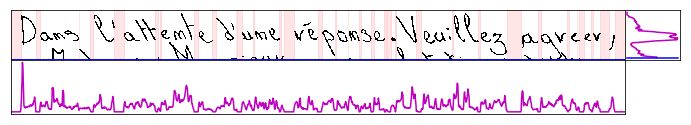
\includegraphics{baseline_segmentation}
					\caption{Badly segmented image, with slanted text}
					\label{fig:baseline_segmentation}
				\end{subfigure}
				\caption[Baseline and tokens]{Detection of the baseline and the tokens in a text image.}
				\label{fig:baseline}
			\end{figure}

		%........................................................................................

		\subsubsection*{Outcome}
			With the above techniques we generated 1000 templates for training, for a total of 50\,000 text examples; we will refer to this dataset as \ds{Template}. It became apparent that this task was appropriately more difficult than the \ds{Collage} dataset, as the validation performance was still improving after 35\,000 steps. However, due to a slow improvement rate, we stopped the training there, as we deemed the validation performance ``good enough'' for an experiment, at \(\AP \simeq 0.76\). Surprisingly though, the performance on the \ds{Test} dataset was essentially zero (\(\AP \simeq 0.007\)). A very close inspection of the generated data, in comparison to the test data, revealed a key difference between the two: the real-world documents are (almost) binarised, while the text from the RIMES database is not (\autoref{fig:template_gray_hist}). Convolutional neural networks should be robust to general appearance changes, especially when random contrast is used as a data augmentation technique. However, knowing that the first filters of CNNs correspond to edge extractors, we hypothesise that the disruption is given by the transitions from foreground (text) to background (white). In the case of RIMES, these are soft edges and only extreme contrast boosts can convert them into hard edges (\autoref{fig:template_gray_example}).

			\begin{figure}
				\begin{subfigure}{\linewidth}
					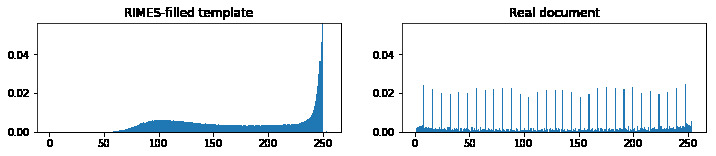
\includegraphics{template_hist}
					\caption[Template histograms]{
						Examples of normalised histograms with the extreme counts removed (0 and 255). The templates filled with text (left) present more shades of gray than a real document (right).  Moreover, only half of real documents present such a structure, the other half being completely binarised, i.e. with a completely empty histogram (after removing the background/foreground extremes).
					}
					\label{fig:template_gray_hist}
				\end{subfigure}
				\begin{subfigure}{\linewidth}
					
\includegraphics[width=.49\linewidth]{binarisation_template}
					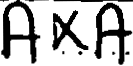
\includegraphics[width=.49\linewidth]{binarisation_real}
					\caption{In addition to being gray, text from the RIMES database has soft edges, while text from real documents has a hard transition from foreground to background.}
					\label{fig:template_gray_example}
				\end{subfigure}
				\caption{Differences between \ds{Template} and \ds{Test}}
				\label{fig:template_gray}
			\end{figure}

			We generated another dataset, \ds{Template_bin}, of same size as \ds{Template}, where we binarised text before pasting it into the documents (\autoref{fig:template_bin_detection}). Given the uniform illumination, a global thresholding technique worked well, with the threshold chosen by Otsu's method. The model trained on this dataset converged after 4500 steps and has a validation \(\AP \simeq 0.83 \). It also generalizes better than previous ones on the \ds{Test} dataset, with an \(\AP \simeq 0.37\).

			\begin{figure}
				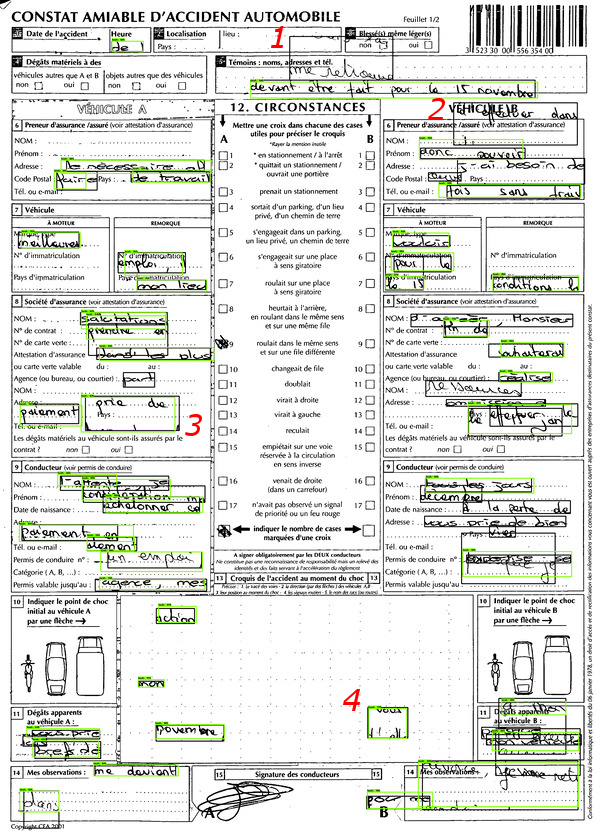
\includegraphics[height=.85\textheight]{template_bin_detection}
				\caption[\ds{Template_bin} example]{Example of template filled with binarised text from the RIMES database. Black shows ground truth boxes, and green the detection result. This particular example also presents some bad ground truth examples, marked by red numbers. Some of them are not detected (1, 2) while some are detected with high precision (3, 4). }
				\label{fig:template_bin_detection}
			\end{figure}

	%----------------------------------------------------------------------------------------
	\subsection{Generator-filled templates}
		As will be apparent from the results of the \FRCNN{} architecture (\autoref{sec:frcnn_results}), the model learnt to predict rather tall bounding boxes which are not representative for real documents. One reason for this is that we used the original height of text lines in order to avoid artefacts of interpolation in resizing. Additionally, the model picked up peculiarities of the training set, such as incorrectly segmented lines.

		%........................................................................................

		\subsubsection*{\ds{Template_gen} dataset}

			To overcome the above limitations, we used our text generator from \autoref{sec:generator} to fill templates as before. It produces coherent and realistic-looking text of given dimensions. This ensures the bounding boxes are always tight and a correct baseline is used for alignment inside the placeholder. Moreover, the height of the text is within the boundaries of the placeholder while keeping the binary distribution of pixels (i.e. avoiding interpolation). The sole possible disadvantage of this method is that we did not enforce a consistent style for all text pieces in a given section. Nevertheless, we realised this should bear a minimal influence on the detection since the algorithm is translation invariant and it scans the image left to right, top to bottom, not following the section order.

		%........................................................................................
		\subsubsection*{Outcome}

			This model was the fastest to converge of all, attaining a validation \(\AP = 0.98\) in approximately 3500 iterations. However, when visually inspecting a small detection sample of validation images at \(\mathit{step} = 3500\), we note a relatively low recall compared to expectations from previous model (\autoref{fig:gen_detection}). This could be explained by the complete separation of validation and training data, the two being generated with completely different text and sets of fonts. Additionally, we also note a higher than usual loss of the classification core, which means that the RPN learnt quickly to propose text-like boxes, but the classification network was not yet sure which ones correspond to handwriting. This is expected to a certain degree since printed and handwritten text are very similar in our documents. Finally, the apparent high performance despite the visually low recall highlights why a more in-depth analysis is needed.

			We further trained the model for another 4000 steps, until the classification loss also converged; the validation precision remained the same. At this point, we tested the model on the \ds{Test} set and noted approximately 10\% improvement over the previous best, with \(\AP = 0.47\).

			\begin{figure}
				% floatrow magic for having sidecaption https://tex.stackexchange.com/a/29144/76755
				\floatbox[{\capbeside\thisfloatsetup{capbesideposition={left,top},capbesidewidth=.48\linewidth}}]{figure}
				{
					\caption[\ds{Template_gen} detection]{Despite reporting almost perfect precision after 3500 steps, a \FRCNN{} model trained on \ds{Template_gen} dataset exhibits quite a low recall that is hard to explain. This small example shows similarly looking text; some of it was detected with maximal confidence, some of it was ignored. Black boxes represent ground truth and are \emph{not} part of the image. }
					\label{fig:gen_detection}
				}
				{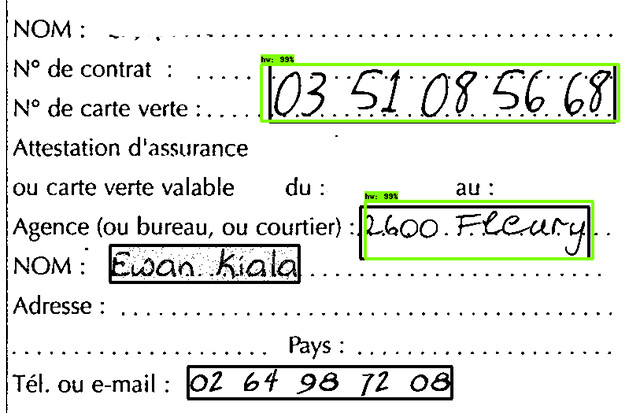
\includegraphics{gen_detection_no}}
			\end{figure}

	%----------------------------------------------------------------------------------------
	\subsection{CTPN test}
		Having proved the feasibility of general object detection architectures for our task, we started seeking further improvements by employing the text-specialised architecture of \CTPN{}. We build upon the previous progress and train directly on the dataset with best results so far, \ds{Template_gen}. The model converged after 10\,000 steps and achieved a validation \(\AP = 0.69\). Despite giving the best results visually on \ds{Test} dataset, it appears to perform worse than the best \FRCNN{} model, with \(\AP = 0.31\).


%========================================================================================


\section{In-depth evaluation}\label{sec:detection_results}
	% this evaluates text detection in 2 simple numbers (P, R), in terms of pixels: http://vision.soic.indiana.edu/papers/textevaluation2000das.pdf

	We have seen in the previous section that different combinations of architectures and training datasets achieve vastly different performances on real data. Moreover, as briefly discussed in \autoref{sec:detection_eval}, it is difficult to quantify them through a single number. This was also confirmed empirically when observing that intermediate models with high \(\AP\) scores gave subpar detections. Therefore, in what follows we will perform a more in-depth analysis of models' performance in the interest of finding the factors that contribute to improvement and choosing the most robust model.

	\Citet{objdet_performance} give an overview of different metrics that can be useful for detailed evaluation of object detection algorithms. We are interested in evaluating both the detection \emph{quantity}, as well as its \emph{quality}. However, these two measures are related, since the detection quantity depends on our quality requirements. We could overcome this tight connection by performing evaluation at a higher level through a \emph{goal-directed} approach. In such a case, the text locating algorithms would be judged by the recognition rate they achieve when coupled with a text recogniser. However, this would introduce another dependency in the system and, to the best of our knowledge, no robust system exists yet for handwriting.

	We reiterate the main concerns for this evaluation:
	\begin{description}
		\item[high recall] A good model should find most of the ground truth boxes.
		\item[precise detection] Bounding boxes that correspond to ground truth should be tight around the text. Note this is different from the overall precision in general (see next point).
		\item[variable general precision] We are forgiving about false positive detections, i.e.\ bounding boxes that do not correspond to any ground truth, since we expect the recogniser to fail on these, thus acting as a filter.
	\end{description}

	\subsection{Faster R-CNN}\label{sec:frcnn_results}
		\urldef{\cocoURL}\url{http://cocodataset.org/#detections-challenge2017}

		We started our training with a model pre-trained for the COCO object detection challenge\footnote{Common Objects in Context \cocoURL}, which claimed an \(\AP \simeq 0.32\). We have reached a similar performance on our \ds{Test} dataset. On the one hand, further improvements should be possible since our task has less classes and less background variation. On the other hand, what we call \emph{background} actually consists of printed text, which is very similar in structure to the handwritten one, especially if both are upper case. We will consider this as a baseline and we will inspect how the training data affects the performance.

		%........................................................................................
		\subsubsection*{Metrics}
			In a first phase, we use the confidence scores to rank the detections and we inspect the variation of recall while varying the score threshold (\autoref{fig:frcnn_results} top). Recall at threshold \(\tau\) is defined as the ratio between the number of true positives and the number of \mbox{ground truth} boxes:
			\[
				R_{\tau} = \frac{\card{\operatorname{TP}_\tau}}{\card{\operatorname{GT}}}.
			\]
			Since we are already filtering by \emph{confidence} score, we consider predicted boxes as true positives when they overlap a ground truth box, regardless of the \(\iou\). This allows even the smallest overlap to count as positive. Therefore, it is mandatory to also look at the distribution of precision values for the same variation of thresholds (\autoref{fig:frcnn_results} middle). Precision at threshold \(\tau\) is defined as the average \(\iou\) of all \emph{positive} predictions \(B^p_i\):
			\[
					P_\tau = \frac{1}{\card{B^p}}~~~ \sum_{B^p_i,\ \operatorname{score}(B^p_i ) > \tau} \iou(B^p_i, B^{gt}_i),
			\]
			where mapping to ground truth of a predicted box \(B^p_i\) happens greedily and in rank order:
			\[
					B^{gt}_i = \argmax_{B^{gt}_j} \iou(B^{gt}_j, B^p_i).
			\]

		%........................................................................................
		\subsubsection*{Results interpretation}
			As expected from the intermediate results, the model trained on the gray-scale dataset \ds{Template} has the lowest recall and precision. However, for the very few boxes that it detects with high confidence (\(c \geq 0.8\)) it also gives very good overlap. This is opposite to the model trained on \ds{Collage}, which seems to have learned to detect the wrong thing, as higher confidence decreases both the recall and the precision.

			The model trained on \ds{Template_bin} gives the most intuitive results as the score threshold influences almost linearly both the recall (downwards) and the precision (upwards). Before our text generator was implemented, we believed this to be the maximum achievable with the given datasets. It was then confirmed by the result of model trained on \ds{Template_gen}, which addresses most of the previous limitations. Therefore, it has better recall at all confidence levels, and better precision in general. There seems to be a small exception for high confidence levels (\(c \geq 0.85\)), where \ds{Template_bin} appears to give tighter bounding boxes. However, this is caused by averaging over a smaller number of instances (see recall curve), which is confirmed by the   average deviation of the mean \(\iou\).

			If we posit that the confidence score bears little importance in our context, we may approach the problem from a different angle, keeping in mind that we want the detection to be as tight as possible around the text. We rank the boxes by their overlap with the mapped ground truth
			%\footnote{The mapping is again done greedily}
			, i.e.\ \(\operatorname{score}(B^p_k) = \iou(B^p_k, B^{gt}_k)\) thus getting a precision-recall curve (\autoref{fig:frcnn_results} bottom).
			In this case it is more evident that the model trained on \ds{Template_gen} is superior to the others since it maintains a higher recall rate while we filter the boxes to be of increasingly higher quality.


	%----------------------------------------------------------------------------------------
	\vspace*{-1em}
	\subsection{Connectionist Text Proposal Network}\label{sec:ctpn_results}
		We evaluate the results of \CTPN{} architecture using the same \ds{Test} dataset and, of course, the same metrics as for \FRCNN{}. These are displayed in \autoref{fig:ctpn_results}. The \CTPN{} model gives very high confidence (\(c \geq 0.9\)) for virtually all the outputted boxes. For this reason, the curves filtered by this score are essentially flat.

		We can argue, based on the middle and bottom plots, that the model performs worse than the best \FRCNN{} model, giving slightly worse overlaps and with less recall. This contradicts a little our intuition. Visualising the results, we observed that the bounding boxes of \FRCNN{} often cut the sides of text while being a little taller, whereas the \CTPN{} makes a better vertical separation while including more white space to the left and right of text. Such differences are difficult to quantify with our chosen measures. Furthermore, we believe the lower recall of \CTPN{} is due to how we assign detections to ground truth. Namely, each predicted box is assigned \emph{uniquely} to the ground truth of highest overlap; other ground truth boxes covered by the same prediction are counted as undetected. This is unfavourable for the model, since it often merges together predictions lying on the same line (\autoref{fig:ctpn_overzealous_merge}), under the control of hyperparameter \(\tau_{gap}\).
		\vspace*{-0.25em}
		\begin{figure}[htb]
			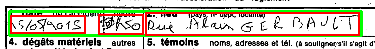
\includegraphics{ctpn_overzealous}
			\caption[\CTPN{} overzealous merging]{The \CTPN{} predicts a single box covering multiple ground truths in the same line.
			While essentially correct,
			%since a good transcription system should be able to handle this detection,
			in our measures only the largest ground truth is counted as detected.
			}
			\label{fig:ctpn_overzealous_merge}
		\end{figure}

		\begin{figure}
			\vspace{-2em}
			\begin{subfigure}{.49\linewidth}
					\caption{\FRCNN{}}\label{fig:frcnn_results}
					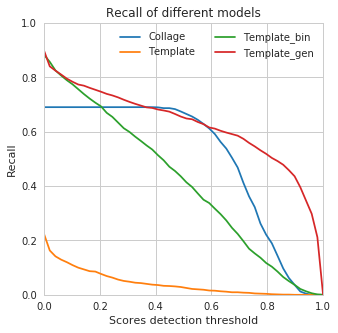
\includegraphics{frcnn_recall_scores}
					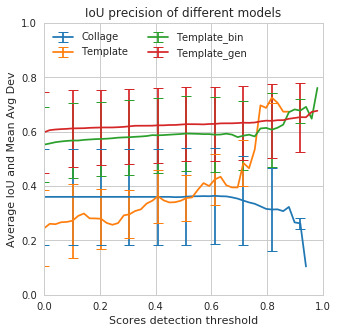
\includegraphics{frcnn_prec_scores}
					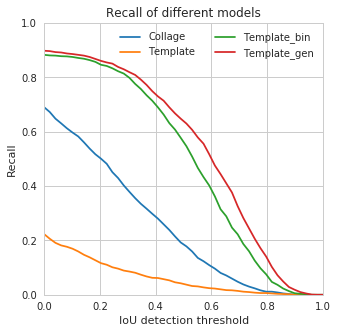
\includegraphics{frcnn_recall_iou}
			\end{subfigure}
			\rulesep
			\begin{subfigure}{.49\linewidth}
					\caption{\CTPN{}}\label{fig:ctpn_results}
					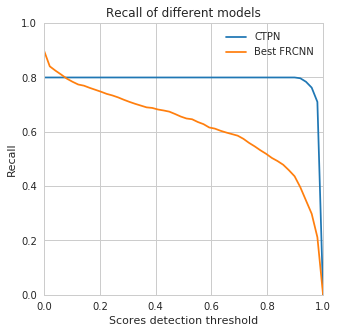
\includegraphics{ctpn_recall_scores}
					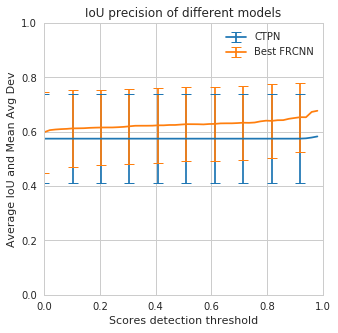
\includegraphics{ctpn_prec_scores.png}
					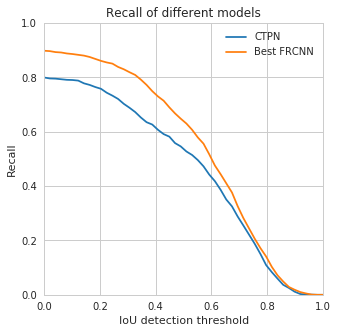
\includegraphics{ctpn_recall_iou}
			\end{subfigure}
			\caption{Text detection results}
		\end{figure}


\bibliography{refs}             % this causes the references to be listed
\bibliographystyle{plainnat}       % see natbib for other possible values

% \include{chapters/appendix}

\end{document}
